\scanpage{24}
\deleted{objets $S$ pour lesquels il existe une suite $\sim$-exacte de \deleted{\unsure{suites}} \inserted{complexes} \deleted{suites du type $S(X)$.} $0\to S\to S(X)\to S^*-0$. [pour le voir, on écrit, si $0\unsure{-|\to}A'-A-A''-0$ est $\sim$-exacte,}

% slanted
\margin{Dorénavant, $\sim$ est exact et ``fidèle''}

\diagram{\begin{tikzcd}[ampersand replacement=\&,column sep=small]
\deleted{0}\arrow[r,dash] \& \deleted{A'}\arrow[r,dash,"\deleted{u}"]\arrow[d,"\deleted{\unsure{i_{A'}u|i_{A'} }}"] \& \deleted{A}\arrow[r,dash,"\deleted{v}"]\arrow[d,"\deleted{i_A}"] \& \deleted{A''}\arrow[r,dash]\arrow[d] \& \deleted{0}\\
\deleted{0}\arrow[r,dash] \& \deleted{T(\unsure{A|A'})}\arrow[r,"\deleted{\unsure{i_A|u}}"'] \& \deleted{\unsure{T(T(A))|TT(A)}}\arrow[r,dash] \& \deleted{\unsure{T(A)^*}}\arrow[r] \& \deleted{0}
\end{tikzcd}}

\figure{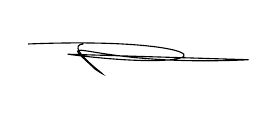
\begin{tikzpicture}[x=1cm,y=1cm]\draw (0,.2).. controls (2.5,.3) and (2.6,-.2) .. (.5,.07)--(2.8,0).. controls (.7,-.1) and (.3,.4) .. (.85,-.12).. controls (1.2,-.35) and (.4,.18) .. (.7,.2);\end{tikzpicture}}

Une $S$-résolution d'un $A\in\mathcal C$ est une résolution \deleted{\illegible{1}} $X$ de $A$, \uline{munie} d'un opérateur d'homotopie \deleted{\illegible{1}} \unsure{$s$} dans le complexe augmenté $0-\unsure{\widetilde A|\bar A}-\widetilde X^0-\widetilde X^1-\widetilde X^{\unsure{2|3}}-\ldots$ i.e. de projections \inserted{splittantes} dans les suites exactes

\[
0-Z^i(X^*)-X^i\to Z^{i+1}(X^*)-0\qquad (i\geq0)
\]

\deleted{\uline{Proposition} \unsure{Soit} $X$ \unsure{une résolution|projectifs}}
\deleted{Un \deleted{application} \inserted{morphisme} \deleted{$\unsure{f}:$ \illegible{1}} $\unsure{\eta|y}:X\to Y$ de $\mathcal C$ est dit \deleted{\unsure{spécial} \unsure{spéciale}} \inserted{effaçant} si \deleted{$\widetilde X-\widetilde Y$ est} pour tout $A\in\mathcal C$, l'image de $\mathrm{Hom}(\widetilde A,\widetilde X)$ dans $\mathrm{Hom}(\widetilde A,\widetilde Y)$ par $u\to\widetilde\eta\,\widetilde u$ est contenue dans l'image de $\mathrm{Hom}(A,Y)$, i.e. si on a un diagramme commutatif}

\diagram{\begin{tikzcd}[ampersand replacement=\&,column sep=large]
\deleted{\mathrm{Hom}(\widetilde A,\widetilde X)}\arrow[r,"\deleted{\unsure{u}\,-\,\widetilde\eta\widetilde u}"]\arrow[dr] \& \deleted{\mathrm{Hom}(\widetilde A,\widetilde Y)}\\
\deleted{\mathrm{Hom}(A,T(X))}\arrow[u,"\deleted{\unsure{\sim}}"'] \& \deleted{\mathrm{Hom}(A,Y)}\arrow[u,"\deleted{\sim}"]
\end{tikzcd}}

% paper watermark: ARGENTINE TYPEWRITER (vertical, partly cropped)
% archive sheet number: 23
